%<dscrpt>Fichier de déclarations Latex à inclure au début d'un élément de cours.</dscrpt>

\documentclass[a4paper]{article}
\usepackage[hmargin={1.8cm,1.8cm},vmargin={2.4cm,2.4cm},headheight=13.1pt]{geometry}

%includeheadfoot,scale=1.1,centering,hoffset=-0.5cm,
\usepackage[pdftex]{graphicx,color}
\usepackage[french]{babel}
%\selectlanguage{french}
\addto\captionsfrench{
  \def\contentsname{Plan}
}
\usepackage{fancyhdr}
\usepackage{floatflt}
\usepackage{amsmath}
\usepackage{amssymb}
\usepackage{amsthm}
\usepackage{stmaryrd}
%\usepackage{ucs}
\usepackage[utf8]{inputenc}
%\usepackage[latin1]{inputenc}
\usepackage[T1]{fontenc}


\usepackage{titletoc}
%\contentsmargin{2.55em}
\dottedcontents{section}[2.5em]{}{1.8em}{1pc}
\dottedcontents{subsection}[3.5em]{}{1.2em}{1pc}
\dottedcontents{subsubsection}[5em]{}{1em}{1pc}

\usepackage[pdftex,colorlinks={true},urlcolor={blue},pdfauthor={remy Nicolai},bookmarks={true}]{hyperref}
\usepackage{makeidx}

\usepackage{multicol}
\usepackage{multirow}
\usepackage{wrapfig}
\usepackage{array}
\usepackage{subfig}


%\usepackage{tikz}
%\usetikzlibrary{calc, shapes, backgrounds}
%pour la présentation du pseudo-code
% !!!!!!!!!!!!!!      le package n'est pas présent sur le serveur sous fedora 16 !!!!!!!!!!!!!!!!!!!!!!!!
%\usepackage[french,ruled,vlined]{algorithm2e}

%pr{\'e}sentation du compteur de niveau 2 dans les listes
\makeatletter
\renewcommand{\labelenumii}{\theenumii.}
\renewcommand{\thesection}{\Roman{section}.}
\renewcommand{\thesubsection}{\arabic{subsection}.}
\renewcommand{\thesubsubsection}{\arabic{subsubsection}.}
\makeatother


%dimension des pages, en-t{\^e}te et bas de page
%\pdfpagewidth=20cm
%\pdfpageheight=14cm
%   \setlength{\oddsidemargin}{-2cm}
%   \setlength{\voffset}{-1.5cm}
%   \setlength{\textheight}{12cm}
%   \setlength{\textwidth}{25.2cm}
   \columnsep=1cm
   \columnseprule=0.5pt

%En tete et pied de page
\pagestyle{fancy}
\lhead{MPSI-\'Eléments de cours}
\rhead{\today}
%\rhead{25/11/05}
\lfoot{\tiny{Cette création est mise à disposition selon le Contrat\\ Paternité-Pas d'utilisations commerciale-Partage des Conditions Initiales à l'Identique 2.0 France\\ disponible en ligne http://creativecommons.org/licenses/by-nc-sa/2.0/fr/
} }
\rfoot{\tiny{Rémy Nicolai \jobname}}


\newcommand{\baseurl}{http://back.maquisdoc.net/data/cours\_nicolair/}
\newcommand{\urlexo}{http://back.maquisdoc.net/data/exos_nicolair/}
\newcommand{\urlcours}{https://maquisdoc-math.fra1.digitaloceanspaces.com/}

\newcommand{\N}{\mathbb{N}}
\newcommand{\Z}{\mathbb{Z}}
\newcommand{\C}{\mathbb{C}}
\newcommand{\R}{\mathbb{R}}
\newcommand{\D}{\mathbb{D}}
\newcommand{\K}{\mathbf{K}}
\newcommand{\Q}{\mathbb{Q}}
\newcommand{\F}{\mathbf{F}}
\newcommand{\U}{\mathbb{U}}
\newcommand{\p}{\mathbb{P}}


\newcommand{\card}{\mathop{\mathrm{Card}}}
\newcommand{\Id}{\mathop{\mathrm{Id}}}
\newcommand{\Ker}{\mathop{\mathrm{Ker}}}
\newcommand{\Vect}{\mathop{\mathrm{Vect}}}
\newcommand{\cotg}{\mathop{\mathrm{cotan}}}
\newcommand{\sh}{\mathop{\mathrm{sh}}}
\newcommand{\ch}{\mathop{\mathrm{ch}}}
\newcommand{\argsh}{\mathop{\mathrm{argsh}}}
\newcommand{\argch}{\mathop{\mathrm{argch}}}
\newcommand{\tr}{\mathop{\mathrm{tr}}}
\newcommand{\rg}{\mathop{\mathrm{rg}}}
\newcommand{\rang}{\mathop{\mathrm{rg}}}
\newcommand{\Mat}{\mathop{\mathrm{Mat}}}
\newcommand{\MatB}[2]{\mathop{\mathrm{Mat}}_{\mathcal{#1}}\left( #2\right) }
\newcommand{\MatBB}[3]{\mathop{\mathrm{Mat}}_{\mathcal{#1} \mathcal{#2}}\left( #3\right) }
\renewcommand{\Re}{\mathop{\mathrm{Re}}}
\renewcommand{\Im}{\mathop{\mathrm{Im}}}
\renewcommand{\th}{\mathop{\mathrm{th}}}
\newcommand{\repere}{$(O,\overrightarrow{i},\overrightarrow{j},\overrightarrow{k})$}
\newcommand{\cov}{\mathop{\mathrm{Cov}}}

\newcommand{\absolue}[1]{\left| #1 \right|}
\newcommand{\fonc}[5]{#1 : \begin{cases}#2 \rightarrow #3 \\ #4 \mapsto #5 \end{cases}}
\newcommand{\depar}[2]{\dfrac{\partial #1}{\partial #2}}
\newcommand{\norme}[1]{\left\| #1 \right\|}
\newcommand{\se}{\geq}
\newcommand{\ie}{\leq}
\newcommand{\trans}{\mathstrut^t\!}
\newcommand{\val}{\mathop{\mathrm{val}}}
\newcommand{\grad}{\mathop{\overrightarrow{\mathrm{grad}}}}

\newtheorem*{thm}{Théorème}
\newtheorem{thmn}{Théorème}
\newtheorem*{prop}{Proposition}
\newtheorem{propn}{Proposition}
\newtheorem*{pa}{Présentation axiomatique}
\newtheorem*{propdef}{Proposition - Définition}
\newtheorem*{lem}{Lemme}
\newtheorem{lemn}{Lemme}

\theoremstyle{definition}
\newtheorem*{defi}{Définition}
\newtheorem*{nota}{Notation}
\newtheorem*{exple}{Exemple}
\newtheorem*{exples}{Exemples}


\newenvironment{demo}{\renewcommand{\proofname}{Preuve}\begin{proof}}{\end{proof}}
%\renewcommand{\proofname}{Preuve} doit etre après le begin{document} pour fonctionner

\theoremstyle{remark}
\newtheorem*{rem}{Remarque}
\newtheorem*{rems}{Remarques}

\renewcommand{\indexspace}{}
\renewenvironment{theindex}
  {\section*{Index} %\addcontentsline{toc}{section}{\protect\numberline{0.}{Index}}
   \begin{multicols}{2}
    \begin{itemize}}
  {\end{itemize} \end{multicols}}


%pour annuler les commandes beamer
\renewenvironment{frame}{}{}
\newcommand{\frametitle}[1]{}
\newcommand{\framesubtitle}[1]{}

\newcommand{\debutcours}[2]{
  \chead{#1}
  \begin{center}
     \begin{huge}\textbf{#1}\end{huge}
     \begin{Large}\begin{center}Rédaction incomplète. Version #2\end{center}\end{Large}
  \end{center}
  %\section*{Plan et Index}
  %\begin{frame}  commande beamer
  \tableofcontents
  %\end{frame}   commande beamer
  \printindex
}


\makeindex
\begin{document}
\noindent

\debutcours{Fonctions d'une variable géométrique :  calcul intégral}{alpha}

 Toutes les fonctions considérées ici seront supposées assez régulières (au moins $\mathcal C^1$). 

\section{Les trois vies de l'intégrale curviligne}
\subsection{Intégrale curviligne}\index{intégrale curviligne}
Une intégrale curviligne associe un nombre à un couple formé par une courbe orientée (notons la $\Gamma$) et une forme différentielle (1-forme) définie sur cette courbe (notons la $\omega$).\newline
Par courbe, on entend ici un ensemble de points c'est à dire le support (trajectoire) d'une courbe paramétrée. Il existera donc une infinité de paramétrisations admissibles de $\Gamma$. Le caractère orienté se traduit par le fait que tous les changements de paramètre sont des fonctions strictement croissantes.\newline
Une forme différentielle est une application.
\begin{displaymath}
 \left\lbrace 
\begin{aligned}
 \Gamma &\rightarrow E^* \\
 m &\rightarrow w(m)
\end{aligned}
\right. 
\end{displaymath}
Pour chaque $m$, $w(m)$ est une forme linéaire c'est à dire que  $\overrightarrow u \rightarrow \omega(m)(\overrightarrow u)$ est linéaire de $E$ dans $\R$.
\begin{prop}[définition de l'intégrale curviligne]
 Soient $\gamma_1$ définie dans $[a_1,b_1]$ et $\gamma_1$ définie dans $[a_2,b_2]$ deux paramétrisations admissibles d'une courbe $\Gamma$, soit $\omega$ une forme différentielle définie sur $\Gamma$ alors :
\begin{displaymath}
 \int_{a_1}^{b_1}\omega(\gamma_1(u))(\overrightarrow{\gamma_1 '}(u))du 
=
 \int_{a_2}^{b_2}\omega(\gamma_2(v))(\overrightarrow{\gamma_2 '}(v))dv 
\end{displaymath}
Ce nombre est appelé \emph{intégrale curviligne de $\omega$ le long de $\Gamma$} et il est noté
\begin{displaymath}
 \int_\Gamma \omega
\end{displaymath}
\end{prop}
\begin{demo}
 Considérons le changement de paramètre admissible $\varphi$ de $[a_1,b_1]$ dans $[a_2,b_2]$ tel que $\gamma_1 = \gamma_2 \circ \varphi$. Le changement de variable $v=\varphi(u)$ dans une des intégrales conduit à l'autre. Ces deux intégrales sont donc égales. 
\end{demo}
\begin{rem}
 Si on change le sens dans lequel la courbe est parcourue (orientation) l'intégrale curviligne est changée en son opposée.
\end{rem}
\begin{prop}[Linéarité]
 Soit $\omega_1$ et $\omega_2$ deux formes différentielles sur une courbe orientée $\gamma$, soit $\lambda\in \R$:
\begin{displaymath}
 \int_\Gamma \lambda \omega_1 = \lambda \int_\Gamma \omega_1
\hspace{1cm}
\int_\Gamma (\omega_1 + \omega_2) = \int_\Gamma \omega_1 + \int_\Gamma \omega_2
\end{displaymath}
\end{prop}
Addition des courbes. Courbes paramétrées $\mathcal C^1$ par morceaux.
\begin{prop}[Additivité et relation de Chasles]
 \begin{displaymath}
 \int_{\Gamma_1 + \Gamma_2} \omega = \int_{\Gamma_1} \omega+ \int_{\Gamma_2} \omega 
\end{displaymath}
\end{prop}

\begin{figure}[h!t]
  \centering
  \subfloat[le long d'un demi-cercle]{\input{C2269_3.pdf_t}} \hspace{2cm}
  \subfloat[le long d'un graphe de fonction]{\input{C2269_4.pdf_t}}
  \caption{Exemples de calcul d'intégrales curvilignes}
  \label{fig:C2269_3_4}
\end{figure}

\begin{exples}
 \begin{enumerate}
 \item Sur le  demi-cercle $\mathcal C$ de centre $O$ de rayon $1$ et orienté de $A$ de coordonnées $(1,0)$ vers $B$ de coordonnés $(-1,0)$ (voir fig \ref{fig:C2269_3_4} a), on considère la forme différentielle 
\begin{displaymath}
 \omega = (x-y^2)dx + x^3dy
\end{displaymath}
On choisit la paramétrisation $\gamma$ définie dans $[0,\pi]$ par $\gamma(t)=O+\cos t \overrightarrow i + \sin t \overrightarrow j = (\cos t, \sin t)$. On a alors $x(\gamma(t))=\cos t$ et $y(\gamma(t))=\sin t$. De plus,
\begin{multline*}
 \overrightarrow{\gamma'}(t)=-\sin t \overrightarrow i + \cos t \overrightarrow j
\Rightarrow
\left\lbrace 
\begin{aligned}
 dx(\gamma(t))(\overrightarrow{\gamma'}(t)) &=  -\sin t \\
 dy(\gamma(t))(\overrightarrow{\gamma'}(t)) &=  \cos t 
\end{aligned}
\right. \\
\Rightarrow
\int_\mathcal C \omega =
\int_0^\pi\left( (\cos t - \sin^2 t)(-\sin t)+\cos^3t\cos t\right)\,dt \\
=\int_0^\pi
\left(-\frac{1}{2}\sin(2t)+\frac{3}{4}\sin t -\frac{1}{4}\sin(3t)
      -\frac{1}{8}\cos(4t) -\frac{1}{2}\cos(2t)-\frac{3}{8}
\right)\,dt 
=\frac{3}{4}-\frac{3\pi}{8}
\end{multline*}

\item 
On considère une fonction $f\in \mathcal C^1([a,b])$ et à valeurs positives. Les courbes orientées $\Gamma_1$, $\Gamma_2$, $\Gamma_3$, $\Gamma_4$ sont définies sur la figure \ref{fig:C2269_3_4} b. On se propose de donner une expression de l'intégrale curviligne de $\omega=-ydx$ le long de la courbe $\Gamma_1+\Gamma_2+\Gamma_3+\Gamma_4$.
\end{enumerate}
\end{exples}

\subsection{Circulation d'un champ de vecteurs}

\index{circulation d'un champ de vecteurs}
\begin{wrapfigure}{l}{9cm}
 \centering
\input{C2269_6.pdf_t}
\caption{Circulation d'un champ de vecteurs.}
\label{fig:C2269_6}
\end{wrapfigure}
Dans un espace euclidien, à chaque champ $\overrightarrow X$ défini sur une courbe $\Gamma$, on peut associer une 1-forme $\omega_c$ définie  par :
\begin{displaymath}
 \forall m\in \Gamma,  \forall \overrightarrow u :\;
\omega_c(m)(\overrightarrow u ) = (\overrightarrow X (m)/ \overrightarrow u)
\end{displaymath}
 On peut alors définir la circulation d'un champ à partir d'une intégrale curviligne.
\begin{defi}[circulation d'un champ]
 Soit $\Gamma$ une courbe orientée et $\overrightarrow X$ un champ de vecteurs défini sur $\Gamma$. La \emph{circulation du champ $\overrightarrow X$ le long de la courbe} $\Gamma$ est $\int_\Gamma \omega_c$. Elle est notée $\int_{\Gamma}\overrightarrow X$.
\end{defi}
\begin{rem}
 La circulation d'un champ vérifie les mêmes propriétés  que l'intégrale curviligne: relation de Chasles vis à vis de la courbe sur laquelle on intègre et linéarité vis à vis du champ.
\end{rem}
\begin{prop}[expression en coordonnées]
 Soit $(O,(\overrightarrow{i},\overrightarrow{i}))$ un repère orthonormé pour lequel $x$ et $y$ désignent les fonctions coordonnées. Soit $\Gamma$ une courbe orientée paramétrée par $\gamma$ définie dans $[a,b]$. On note $u=x\circ \gamma$, $v=y\circ \gamma$ les coordonnées de $\gamma$ et $A$, $B$ celles de $\overrightarrow X$. Alors
\begin{align*}
 &\forall m\in \Gamma, \overrightarrow X(m) = A(m)\overrightarrow i + B(m)\overrightarrow j\hspace{0.5cm}
\omega_c(m) = A\,dx +B\,dy \\
& \int_\Gamma \overrightarrow X = \int_a^b \left(A(\gamma(t)u'(t)+B(\gamma(t)v'(t) \right)\,dt  
\end{align*}
\end{prop}
\begin{demo}
 à rédiger
\end{demo}

\subsection{Flux d'un champ de vecteurs}
\begin{wrapfigure}{l}{9.5cm}
 \centering
\input{C2269_7.pdf_t}
\caption{Flux sortant}
\label{fig:C2269_7}
\end{wrapfigure}

\index{flux d'un champ de vecteurs à travers une courbe}
Dans un espace euclidien, à chaque champ $\overrightarrow X$ défini sur une courbe $\Gamma$, on peut associer des formes différentielles $\omega^s$ et $\omega_e$ définies par :
\begin{displaymath}
 \forall m\in \Gamma,  \forall \overrightarrow u :\;
\left\lbrace 
\begin{aligned}
 \omega^e(m)(\overrightarrow u ) &= \det(\overrightarrow u,\overrightarrow X (m))\\
 \omega^s(m)(\overrightarrow u ) &= \det(\overrightarrow X (m),\overrightarrow u)
\end{aligned}
\right. 
\end{displaymath}
\index{flux entrant}\index{flux sortant}
 On peut alors introduire ( avec une intégrale curviligne) les notions de flux entrant et sortant d'un champ à travers une courbe.
\begin{defi}[flux d'un champ]
 Soit $\Gamma$ une courbe orientée et $\overrightarrow X$ un champ de vecteurs défini sur $\Gamma$ dans un plan euclidien. Le \emph{flux entrant} noté $\Phi^e_\Gamma (\overrightarrow X)$ et \emph{flux sortant} noté $\Phi^s_\Gamma (\overrightarrow X)$ sont définis par :
\begin{displaymath}
 \Phi^e_\Gamma (\overrightarrow X)=\int_\Gamma \omega^e,\hspace{1cm}
 \Phi^s_\Gamma (\overrightarrow X)=\int_\Gamma \omega^c
\end{displaymath}
\end{defi}

\begin{rems}
 \begin{itemize}
  \item Un flux vérifie les mêmes propriétés que l'intégrale curviligne: relation de Chasles vis à vis de la courbe sur laquelle on intègre et linéarité vis à vis du champ.
  \item  Les flux entrant et sortant sont opposés. Le terme \og entrant\fg\, se justifie en décidant d'un sens direct pour une orientation des courbes. Un courbe paramétrée est dite \emph{directe} lorsqu'elle tourne dans le sens trigonométrique. Par exemple dans la figure \ref{fig:C2269_7}, la courbe orientée est directe, le déterminant $\det(\overrightarrow{X}(\gamma(t),\overrightarrow{\gamma'}(t))$ est positif donc le flux sortant est positif. Pour une courbe fermée, si $\overrightarrow X$ représente la vitesse d'un écoulement, ce flux sortant représente la quantité de matière qui sort de la courbe. 
 \end{itemize}
\end{rems}
\begin{prop}[expression en coordonnées]
 Soit $(O,(\overrightarrow{i},\overrightarrow{i}))$ un repère orthonormé pour lequel $x$ et $y$ désignent les fonctions coordonnées. Soit $\Gamma$ une courbe orientée paramétrée par $\gamma$ définie dans $[a,b]$. On note $u=x\circ \gamma$, $v=y\circ \gamma$ les coordonnées de $\gamma$ et $A$, $B$ celles de $\overrightarrow X$. Alors
\begin{align*}
 &\forall m\in \Gamma, \overrightarrow X(m) = A(m)\overrightarrow i + B(m)\overrightarrow j\hspace{0.5cm}
\omega^s(m) = -B\,dx + A\,dy \\
& \int_\Gamma \overrightarrow X = \int_a^b \left(-B(\gamma(t)u'(t)+ A(\gamma(t)v'(t) \right)\,dt  
\end{align*}
\end{prop}
\begin{demo}
 \begin{displaymath}
  \omega^s = 
\begin{vmatrix}
 A & dx \\ B & dy
\end{vmatrix}
= -B\,dx + A\,dy
 \end{displaymath}
\end{demo}

\subsection{Formes fermées, exactes et notions associées pour les champs}
\subsubsection{Formes exactes}
\index{lacet}\index{forme différentielle exacte}
\begin{wrapfigure}{r}{8cm}
 \centering
\input{C2269_5.pdf_t}
\caption{Un lacet est une courbe fermée}
\label{fig:C2269_5}
\end{wrapfigure}
 Un \emph{lacet} est le support d'une courbe paramétrée périodique et assez régulière. Une forme différentielle $\omega$ est dite \emph{exacte} lorsqu'il existe une fonction $f$ telle que 
\begin{displaymath}
 \omega = df
\end{displaymath}
\begin{prop}
 Soit $\omega=df$ une forme différentielle exacte et $\Gamma$ une courbe orientée de $A$ à $B$ alors :
\begin{displaymath}
 \int_\Gamma \omega = f(B) -f(A)
\end{displaymath}
En particulier, l'intégrale curviligne d'une forme exacte le long d'un lacet ($A=B$) est nulle.
\end{prop}
\begin{demo}
 Soit $\gamma$ définie dans $[a,b]$ une paramétrisation de $\Gamma$ et $\varphi = f\circ \gamma$. On a alors:
\begin{displaymath}
 \forall t\in [a,b], \varphi'(t) = df(\gamma(t))(\overrightarrow{\gamma'}(t))
\Rightarrow
\int_\Gamma \omega = \int_a^b df(\gamma(t))(\overrightarrow{\gamma'}(t))\,dt = \int_a^b \varphi'(t)\,dt=\varphi(b)-\varphi(a)=f(B)-f(A)
\end{displaymath}
\end{demo}
Lorsque une forme différentielle est attachée à un champ pour un calcul de circulation ou de flux, son caractère exact définit une propriété du champ qui prend un nom particulier résumé dans le tableau suivant\index{potentiel scalaire} \index{potentiel vecteur}
\begin{center}
\renewcommand{\arraystretch}{1.5}
\newcolumntype{M}[1]{>{\centering}m{#1}}
\begin{tabular}{|M{4cm}|M{4cm}|M{4cm}|} \hline
 la forme différentielle $\omega$ est exacte &
 le champ $\overrightarrow X$ dérive d'un potentiel scalaire &
 le champ $\overrightarrow X$ dérive d'un potentiel vecteur \tabularnewline
$\Updownarrow$ & $\Updownarrow$ & $\Updownarrow$ \tabularnewline
 il existe $f$ tel que $\omega = df$ &
 il existe $f$ tel que $\overrightarrow X = \grad f$ &
 il existe $\overrightarrow P$ tel que $\overrightarrow X = \overrightarrow{\nabla}\wedge \overrightarrow P$ \tabularnewline
$\Downarrow$ & $\Downarrow$ & $\Downarrow$ \tabularnewline
 l'intégrale curviligne de $\omega$ le long d'un chemin ne dépend que des extrémités &
 la circulation de $\overrightarrow X$ le long d'un chemin ne dépend que des extrémités &
 le flux de $\overrightarrow X$ le long d'un chemin ne dépend que des extrémités \tabularnewline \hline
\end{tabular}
\end{center}
\index{opérateur nabla}
L'opérateur $\overrightarrow{\nabla}$ appelé \emph{opérateur nabla} est un opérateur vecteur. On étend l'espace en un espace euclidien de dimension 3, on pose alors:
\begin{displaymath}
 \overrightarrow{\nabla} = \frac{\partial}{\partial x}\overrightarrow i +
 \frac{\partial}{\partial y}\overrightarrow j +
\frac{\partial}{\partial z}\overrightarrow k
\end{displaymath}
Le potentiel vecteur est dirigé par le troisième vecteur de base $\overrightarrow P = f\overrightarrow k$ et
\renewcommand{\arraystretch}{1.5}
\begin{displaymath}
 \overrightarrow{\nabla}\wedge \overrightarrow P
=\begin{pmatrix}
  \frac{\partial}{\partial x}\\\frac{\partial}{\partial y}\\\frac{\partial}{\partial z}
 \end{pmatrix}
\wedge
\begin{pmatrix}
 0\\0\\f
\end{pmatrix}
=
\begin{pmatrix}
\frac{\partial f}{\partial y}\\ -\frac{\partial f}{\partial x}\\0
\end{pmatrix}
= \frac{\partial f}{\partial y}\overrightarrow i - \frac{\partial f}{\partial x}\overrightarrow j
\end{displaymath}
\begin{rem}\index{champ conservatif}
 Le flux d'un champ qui dérive d'un potentiel vecteur à travers un lacet est nul. On parle de champ \emph{conservatif} car cette propriété traduit le fait que si le champ est un champ de vitesse d'un écoulement, la quantité de matière à l'intérieur d'un lacet est constante, la quantité de matière qui entre est compensée par celle qui sort.
\end{rem}

\subsubsection{Formes fermées.}
D'après le théorème de Schwarz, si $\omega=Adx+Bdy = df$ est une forme différentielle $\mathcal C^1$ exacte, les dérivées croisées sont égales 
\begin{displaymath}
\frac{\partial A}{\partial y}=\frac{\partial^2 f}{\partial y\partial x}=\frac{\partial^2 f}{\partial x\partial y}=\frac{\partial B}{\partial x} 
\end{displaymath}
La réciproque n'est pas vraie. La forme du domaine joue un rôle capital. On précise le nom donné aux formes vérifiant cette propiété et on indique une hypothèse commode assurant la réciproque.
\begin{defi}\index{forme différentielle fermée}
 Une forme différentielle $\omega= Adx +Bdy$ est dite \emph{fermée} si et seulement si :
\begin{displaymath}
 \frac{\partial A}{\partial y} = \frac{\partial B}{\partial x}  
\end{displaymath}
\end{defi}
\begin{demo}
 Il convient de vérifier que cette définition est indépendante du choix du système de coordonnées. L'étude de cette démonstration n'est pas conseillée en première lecture. Elle revient à \href{\baseurl C6308.pdf}{l'indépendance de la différentielle d'une 1-forme vis à vis du système de coordonnées}.
\end{demo}
\begin{wrapfigure}{l}{8cm}
 \centering
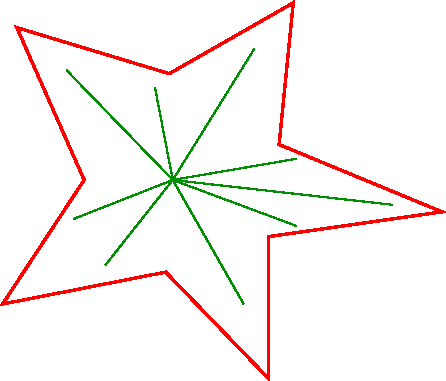
\includegraphics{C2269_8.pdf}
\caption{Partie étoilée}
\label{fig:C2269_8}
\end{wrapfigure}

 La réciproque n'est pas toujours vraie et dépend du domaine $\Omega$ sur lequel la forme est définie. Par exemple 
\begin{displaymath}
 \omega = -\frac{\sin \theta}{\rho} dx +\frac{\cos \theta}{\rho}dy = -\frac{y}{x^2+y^2}dx + \frac{x}{x^2+y^2}dy
\end{displaymath}
est $\mathcal C^1$ dans le plan privé de l'origine.  Elle est fermée car on vérifie par le calcul que les deux dérivées sont égales à $\frac{y^2-x^2}{(x^2+y^2)^2}$. Elle n'est pas exacte. Pour le vérifier, on son intégrale curviligne le long du cercle unité. On trouve $2\pi$ ce qui est impossible pour une forme exacte. Cette forme est présentée comme $d\theta$ mais ce nom est bien mal choisi car il ne peut exister une telle fonction. On retrouve encore une fois la malédiction du logarithme.\index{malédiction du logarithme}

\index{partie étoilée}
\begin{defi}
 On dira qu'une partie $\Omega$ d'un plan est étoilée lorsqu'il existe un point $O\in \Omega$ tel que, pour tout point $m\in \Omega$, le segment $[O,m]$ est inclus dans $\Omega$.
\end{defi}
\index{lemme de Poincaré}
\begin{thm}[Lemme de Poincaré]
Lorsque $\Omega$ est une partie étoilée d'un plan, toute 1-forme fermée de classe $\mathcal C^1$ dans $\Omega$  est exacte. 
\end{thm}
\begin{demo}
 Voir \href{\baseurl C6308.pdf}{Fonctions d'une vaiable géométrique : démonstrations}.
\end{demo}

\begin{rems}
\begin{itemize}
 \item Toute partie convexe est étoilée car \emph{tous} les segments entre deux points quelconques de $\Omega$ sont inclus dans $\Omega$.
\item On peut reformuler le lemme de Poincaré de la manière suivante. Soit $A$ et $B$ deux fonctions $\mathcal C^1(\Omega)$ (avec $\Omega$ étoilé) telles que 
\begin{displaymath}
 \frac{\partial A}{\partial y} = \frac{\partial B}{\partial x} 
\Rightarrow \exists f\in \mathcal C^2(\Omega) \text{ tq }
 \left\lbrace
\begin{aligned}
 \frac{\partial f}{\partial x}=& A \\
 \frac{\partial f}{\partial y}=& b 
\end{aligned}
 \right. 
\Leftrightarrow Adx+bdy = df
\end{displaymath}
\item Il n'est pas nécessaire que $\Omega$ soit étoilé pour que $\omega$ fermée entraine $\omega$ exacte. Ce qu'il faut absolument éviter c'est la présence d'un \og trou\fg.
\end{itemize}
\end{rems}



\section{Intégrale dans un plan}
\subsection{Intégrer quoi ? et où ?}
On doit intégrer des "densités" sur de "bons" convexes. Un physicien dirait "sommer de petits éléments de surface". \index{cahier des charges d'une intégrale} Le "cahier des charges d'une intégrale" doit être satisfait. On doit donner du sens et vérifier les propriétés usuelles : additivité vis à vis du domaine d'intégration (relation de Chasles), linéarité par rapport à ce qu'on intègre, positivité, cohérence vis à vis de configurations élémentaires (calculs d'aire). Comme dans le cas des fonctions d'une variable réelle, un lien existe entre intégration et dérivation mais il est pris ici comme \emph{définition} de l'intégrale d'un variable géométrique dans un plan.\newline
L'objet mathématique adéquat pour la notion de densité est la 2-forme différentielle présentée dans la section suivante. 
\subsection{2-formes différentielles}
\index{2-forme différentielles}
\begin{defi}[2-forme différentielle]
 Une 2-forme différentielle sur un domaine $U$ est un champ de formes bilinéaires alternées.
\end{defi}
\begin{propdef}
 Soit $E$ un $\R$-espace vectoriel de dimension $2$. Pour toutes formes linéaires $\alpha$ et $\beta$, on définit $\alpha\wedge \beta$ par :
\begin{displaymath}
 \forall(x,y)\in \R^2,\; (\alpha\wedge \beta)(x,y)=
\begin{vmatrix}
 \alpha(x)&\alpha(y)\\ \beta(x) & \beta(y)
\end{vmatrix}
\end{displaymath}
alors $\alpha\wedge \beta$ est une forme bilinéaire alternée.
\end{propdef}
\begin{demo}
 La démonstration est immédiate d'après les propriétés du déterminant.
\end{demo}
Si $\alpha$ et $\beta$ sont les formes coordonnées dans une base orthonormée directe, $\alpha\wedge \beta=\det$. Comme l'espace des formes bilinéaires alternées est de dimension $1$ et que $\det$ en est une base. Toute 2-forme différentielle peut s'écrire
\begin{displaymath}
 fdx\wedge dy
\end{displaymath}
où $f$ est une fonction définie dans le domaine.
\subsection{Différentielle}
On a déjà introduit la notion de différentielle d'une fonction $f$, c'est une forme différentielle notée $df$. On dira maintenant $1$-forme au lieu de forme différentielle. On va définir de manière un peu analogue la différentielle d'une $1$-forme $\omega$ qui est notée $d\omega$. C'est une 2-forme. 
\begin{prop}
 Soit $(x,y)$ et $(u,v)$ deux systèmes de coordonnées et 
\begin{displaymath}
 \omega = A dx + B dy = U du + Vdv
\end{displaymath}
une 1-forme. Alors :
\begin{displaymath}
 \left( -\frac{\partial A}{\partial y}+\frac{\partial B}{\partial x}\right)dx\wedge dy =
 \left( -\frac{\partial U}{\partial v}+\frac{\partial V}{\partial u}\right)du\wedge dv 
\end{displaymath}
Cette 2-forme est notée $d\omega$.
\end{prop}
\begin{demo}
 L'étude de cette démonstration n'est pas conseillée en première lecture. Elle est présentée dans un document rassemblant \href{\baseurl C6308.pdf}{les démonstrations des résultats relatifs aux fonctions d'une variable géométrique}.
\end{demo}
\begin{rem}
 Ceci justifie la définition de la notion de forme fermée en la rendant indépendante du système de coordonnées choisi. Il est facile de vérifier que $ddf=0$.
\end{rem}

\subsection{Définition}
\begin{propdef}
 Soit $\Omega$ une "bonne" partie convexe. Pour toute 2-forme $fdx\wedge dy$ définie dans $\Omega$, il existe des 1-formes $\omega$ (dites \emph{primitives}) telles que $d\omega = f dx\wedge dy$. L'intégrale sur le domaine $\Omega$ de la 2-forme $fdx\wedge dy$ est \emph{défini} par
\begin{displaymath}
 \int_\Omega f dx\wedge dy = \int_{\partial \Omega}\omega
\end{displaymath}
où $\partial \Omega$ désigne le \emph{bord} convenablement orienté de $\Omega$.
\end{propdef}
\index{bord d'un domaine}
Cette définition pose plusieurs problèmes : existence des 1-formes \og primitives\fg, indépendance de la valeur de l'intégrale vis à vis du choix de la 1-forme. Il faut ensuite vérifier le cahier des charges annoncé au début.\newline
\index{la formule de Green-Riemann}Il est remarquer que cette définition est le plus souvent présentée dans d'autres cours comme \emph{la formule de Green-Riemann}
\subsubsection{Existence d'une 1-forme primitive}
Ce point sera prouvé plus loin en donnant explicitement de telles formes primitives. D'abord dans la section sur la positivité puis dans celle sur le théorème de Fubini.
\subsubsection{Indépendance vis à vis de la 1-forme}
Toute partie convexe est étoilée donc toute 1-forme fermée définie sur $\Omega$ est exacte. C'est en particulier le cas pour $\omega_1 -\omega_2$ où $\omega_1$ et $\omega_2$ sont des 1-formes primitives de la 2-forme donnée. L'intégrale curviligne le long du lacet $\partial \Omega$ est donc nulle ce qui assure l'indépendance du nombre obtenu vis à vis de la forme primitive choisie.
\subsubsection{Calculs d'aires}
\index{aire}
\begin{wrapfigure}{l}{10cm}
 \centering
  \input{C2269_2.pdf_t}
  \caption{Aire balayée par un rayon vecteur}
  \label{fig:C2269_2}
\end{wrapfigure}
L'aire d'un domaine du plan $\Omega$ est l'intégrale sur $\Omega$ du déterminant $dx\wedge dy$.\newline
On se propose d'utiliser la définition pour calculer des aires dans des cas particuliers significatifs afin de valider la cohérence de cette définition. On utilisera la liberté qui nous est donnée dans le choix d'une forme primitive
\begin{displaymath}
 d(xdy)=d(-ydx)=\frac{1}{2}(-ydx + xdy)
\end{displaymath}
Calculons d'abord l'aire balayée par un rayon vecteur.\index{aire balayée par le rayon vecteur} On en déduira l'aire d'un disque.\newline
On utilise ici $\omega=\frac{1}{2}(-ydx + xdy)$ qui peut s'écrire de mainère plus vectorielle:
\begin{displaymath}
 \omega(m)(\overrightarrow u)=\frac{1}{2}\det(\overrightarrow{om},\overrightarrow u)
\end{displaymath}
Seule la partie en $\Gamma_2$ intervient donc dans le calcul
\begin{displaymath}
 \mathcal{A}(t_1)=\int_{\Gamma_2} \omega = \frac{1}{2}\int_{t_0}^{t_1}\det(\overrightarrow{Of(t)},\overrightarrow{f'}(t))\,dt
= \frac{1}{2}\int_{t_0}^{t_1}\rho^2(t)\theta'(t)\,dt \text{avec}
f(t)=O+\rho(t)\overrightarrow{e_{\theta(t)}}
\end{displaymath}
Dans le cas d'un disque $\rho$ est constant égal au rayon $R$, en intégrant de $0$ à $2\pi$ on trouve bien $\pi R^2$.\index{aire d'un disque}. On retouve aussi la \emph{vitesse aréolaire} \index{vitesse aréolaire} $\mathcal A'(t)=\rho^2\theta'$ qui intervient dans les mouvements à accélération centrale.\index{mouvement à accélération centrale} Un mouvement est à accélération centrale si et seulement si il est paramétré à un coefficient multiplicatif près par l'aire balayée.\newline
Le second exemple est l'aire au dessous du graphe d'une fonction. On en déduit l'aire d'un rectangle.

\subsubsection{Additivité}
\begin{wrapfigure}{l}{8cm}
 \centering
 \input{C2269_9.pdf_t}
 \caption{Additivité des domaines}
 \label{fig:C2269_9}
\end{wrapfigure}
Soit $U$ et $U'$ deux convexes d'intersection $\Omega$ non vide et de bords $\partial U$ et $\partial U'$. Soit $f\,dx\wedge dy$ une 2-forme définie dans $U\cup U'$ et $\omega$ une forme primitive. Il est clair que $U\cup U'$ est étoilée par rapport à un point quelconque de l'intersection. Deux formes primitives quelconques auront donc la même intégrale le long d'un lacet. On peut remarquer aussi que $\Omega$ est convexe.\newline
 Les parties $U_1$ et $U'_1$ sont les complémentaires respectivement de $\Omega$ dans $U$ et $U'$. On introduit des arcs $\Gamma_1$ et $\Gamma_2$ comme sur la figure. Ces arcs constituent le bord de $\Omega$. On peut alors décomposer :
\begin{displaymath}
 \int_{\partial U}\omega = 
\underset{=\int_{\partial U_1}\omega}{\underbrace{\int_{\Gamma}\omega + \int_{\Gamma_1}\omega}} +
\underset{\int_{\partial \Omega}\omega}{\underbrace{\int_{ -\Gamma_1}\omega + \int_{- \Gamma'_1}\omega}}
\end{displaymath}
On obtient une formule analogue pour $U'$. On peut donc en déduire :
\begin{displaymath}
 \int_{U\cup U'}f\,dx\wedge dy + \int_{\Omega}f\,dx\wedge dy = \int_{U}f\,dx\wedge dy + \int_{U'}f\,dx\wedge dy
\end{displaymath}
Ces formules permettent de calculer des intégrales sur des domaines qui ne sont pas convexes.

\subsubsection{Positivité}
\begin{wrapfigure}{r}{7cm}
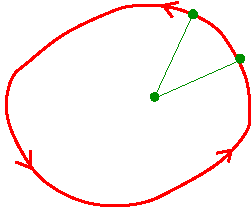
\includegraphics{C2269_10.pdf}
 \caption{Bord orienté positivement}
 \label{fig:C2269_10}
\end{wrapfigure}

La positivité est indispensable pour faire de l'analyse avec des intégrales. Combinée avec la linéarité elle permet d'intégrer des inégalités. Dans la présentation de ce cours à base de 2-formes, l'orientation est très importante. Elle intervient de deux manères : dans la définition des 2-formes positives et dans l'orientation du bord.\newline
L'espace est orienté. Ceci induit une 2-forme particulière attachée au déterminant. Une 2-forme est dite positive lorsqu'elle s'écrit $f\,dx\wedge dy$ où $f$ est une fonction à valeurs positives. Les fonctions $x$ et $y$ sont les fonctions coordonnées attachées à un repère orthonormé direct et $dx\wedge dy$ est la 2-forme déterminant.\newline
Le bord du domaine convexe d'intégration est orienté positivement c'est à dire dans le sens trigonométrique. Cela se traduit commodément lorsque le bord est paramétré de manière polaire en prenant le pôle à l'intérieur de $\Omega$. Une telle paramétrisation est de la forme
$t\rightarrow O+ r_{\Omega}(t)\overrightarrow{e}_{\theta((t)}$ pour $t$ entre $t_0$ et $t_0$ avec $\theta'(t)\geq 0$.\newline
La fonction $f$ se factorise à travers les fonctions du repère polaire. Il existe une fonction $\varphi_{\mathcal P}$ telle que 
\begin{displaymath}
 \forall m\in \Omega, f(m)= \varphi_{\mathcal P}(\rho(m),\theta(m))
\end{displaymath}
On peut alors choisir une forme primitive particulière
\begin{displaymath}
 \omega = \left(\int_0^\rho r \varphi_{\mathcal P}(r,\theta)  \right) \,d\theta
\Rightarrow
d\omega = \rho \varphi_{\mathcal P}(\rho,\theta) \,d\rho\wedge d\theta
=f\rho \,d\rho\wedge d\theta = f\,dx\wedge dy
\end{displaymath}
d'où
\begin{displaymath}
 \int_\Omega f\,dx\wedge dy =
\int_{\partial \Omega} \omega=
\int_{t_0}^{t_1}\left(\int_{0}^{r_{\Omega}(t)}
\underset{\geq 0}{\underbrace{r\varphi_{\mathcal P}(r,\theta)}}\,d\theta
 \right)
\underset{\geq 0}{\underbrace{\theta'(t)}}dt \geq 0 
\end{displaymath}


\subsection{Intégrales doubles. Théorème de Fubini}
\index{intégrale double}\index{théorème de Fubini}
\begin{figure}[h!t]
  \centering
  \input{C2269_1.pdf_t}
  \caption{Tranches "verticales"}
  \label{fig:C2269_1}
\end{figure} 
Ici $\Omega$ est une "bonne" partie convexe du plan, $f$ une fonction définie sur $\Omega$. On se propose d'exprimer
\begin{displaymath}
 \int_\Omega f\,dx\wedge dy
\end{displaymath}
 à l'aide d'une double intégrale.

Pour cela, on découpe $\Omega$ en "tranches verticales" et on explicite une 1-forme primitive de $f\,dx\wedge dy$.\newline
Le fait que $\Omega$ soit une "bonne" partie convexe du plan se traduit en particulier par l'existence d'un rectangle ($[a,b]\times[c,d]$) contenant $\Omega$ et par l'existence de fonctions numériques $\gamma$ et $\delta$ définies dans $[a,b]$ telles que (voir Fig \ref{fig:C2269_1}):
\begin{displaymath}
 \Omega = \bigcup_{u\in[a,b]}\{u\}\times [\gamma(u),\delta(u)]
\end{displaymath}
Ce découpage permet de définir aussi une fonction $A$ dans $\Omega$  par :
\begin{displaymath}
 A(m) = \int_{\gamma(x(m))}^{y(m)}f((x(m),v))\,dv
\end{displaymath}
et une forme différentielle $\omega_v = -Adx$. La définition même de $A$ induit $d\omega_v = f\, dx dy$ car :
\begin{displaymath}
 \dfrac{\partial A}{\partial y}(m)=f(m)
\end{displaymath}
Il reste à évaluer l'intégrale curviligne de $\omega_v$ sur le bord orienté $\Gamma$ du convexe.
\begin{displaymath}
 \int_\Gamma \omega_v = \int_{\Gamma_1}\omega_v + \int_{\Gamma_2}\omega_v - \int_{\Gamma_3}\omega_v - \int_{\Gamma_4}\omega_v
\end{displaymath}
Notons $\gamma_1$, $\gamma_2$, $\gamma_3$, $\gamma_4$ des paramétrisations respectives des courbes $\Gamma_1$, $\Gamma_2$, $\Gamma_3$, $\Gamma_4$.
\begin{itemize}
 \item Les vitesse $\overrightarrow{\gamma_1^\prime}(t)$ et $\overrightarrow{\gamma_2^\prime}(t)$ sont dans la direction de $\overrightarrow{j}$ donc :
\begin{displaymath}
 dx_{\gamma_1(t)}(\overrightarrow{\gamma_1^\prime}(t)) = dx_{\gamma_2(t)}(\overrightarrow{\gamma_2^\prime}(t)) = 0
\end{displaymath}
\item Lorsque $m\in \Gamma_2$, $A(m)=0$ car $y(m)$ est alors la borne du bas de l'intégrale définissant $A$ donc
\begin{displaymath}
 dx_{\gamma_1(t)}(\overrightarrow{\gamma_2^\prime}(t)) = 0
\end{displaymath}
 \item Seul $\Gamma_3$ contribue à l'intégrale. Lorsque $m\in \Gamma_3$ il est sur le bord supérieur du convexe,
\begin{align*}
 u\in[a,b] , \gamma_3(u) &= (u,\delta(u)) \\
A(\gamma_3(u)  &= \int_{\gamma(u)}^{\delta(u)} f((u,v))dv \\
dx_{\gamma_3(u)}(\overrightarrow{\gamma_3^\prime}(t)) &= 1
\end{align*}
 les deux signes - se compensent et on obtient finalement
\end{itemize}
\begin{displaymath}
 \int_\Omega f\,dxdy = \int_{a}^{b}\left(\int_{\gamma(u)}^{\delta(u)} f((u,v))dv \right) du
\end{displaymath}

\subsection{Changement de système de coordonnées}
Il s'agit d'exprimer l'intégrale d'une 2-forme sur un domaine géométrique à l'aide d'un système de fonctions coordonnées. Notons $\mathcal D$ le domaine géométrique et $\Omega$ la 2-forme.\newline
La définition du produit extérieur donné plus haut dans le paragraphe sur les deux formes est commode dans ce cadre. Notons $\mathcal C = (x,y)$ et $\mathcal S=(u,v)$ les deux systèmes de coordonnées. On peut relier simplement $dx\wedge dy$ et $du\wedge dv$ avec le jacobien noté $J$.\index{jacobien} 
\begin{displaymath}
 \left. 
\begin{aligned}
 du &= \frac{\partial u}{\partial x}dx + \frac{\partial u}{\partial y}dy \\ 
 dv &= \frac{\partial v}{\partial x}dx + \frac{\partial v}{\partial y}dy 
\end{aligned}
\right\rbrace \Rightarrow
du\wedge dv = \left(
 \frac{\partial u}{\partial x}\frac{\partial v}{\partial y}
- \frac{\partial u}{\partial y}\frac{\partial v}{\partial x}
 \right) dx\wedge dy = J dx\wedge dy
\end{displaymath}
Comme toute 2-forme peut s'écrire $\Omega = fdx\wedge dy$, où $f$ est une fonction définie dans $\mathcal D$, tant que l'on reste au niveau géométrique, cela est suffisant. On a seulement changé de base pour l'espace des deux formes.
\begin{displaymath}
 \Omega = fdx\wedge dy = \frac{f}{J}du\wedge dv
\end{displaymath}
 Si l'on veut passer à une intégrale double, il faut préciser les données à travers le système choisi.\footnote{Un point de vue platonicien. Les objets géométriques sont dans la caverne. On n'y accèdent qu'à travers les ombres qu'ils portent.}\newline
Introduisons une partie de $\R^2$ notée $\mathcal I_{\mathcal S}(\mathcal D)$ désignée comme l'image de $U$ à travers le système $\mathcal S$.
\begin{displaymath}
 \mathcal I_{\mathcal S}(\mathcal D)=
\left\lbrace (u(m),v(m)), m\in \mathcal D \right\rbrace 
\end{displaymath}
On peut introduire une fonction notée $\varphi_{\mathcal S}$ définie sur $\mathcal I_{\mathcal S}(\mathcal D)$ qui factorise $f$ à travers $u$ et $v$.
\begin{displaymath}                                                                                                                                                       
\forall m\in \mathcal D:\; f(m)=\varphi_{\mathcal S}(u(m),v(m))\text{ avec } (u(m),v(m))\in \mathcal I_{\mathcal S}(\mathcal D)
\end{displaymath}
On peut factoriser ainsi toute fonction à travers un système de coordonnées quelconque:
\begin{displaymath}
\forall m\in \mathcal D:\; f(m)=\varphi_{\mathcal S}(u(m),v(m))= \varphi_{\mathcal C}(x(m),y(m))
\end{displaymath}
Lorsque tout est exprimé à travers un système de coordonnées et que l'image du domaine à travers ce système est assez bien connue pour que l'on puisse le découper, on peut alors passer à une intégrale double.
\end{document}
